\chapter{Introduction}

\textbf{\color{red} This chapter is approximately complete, but the conclusions section and augmented feedback background section do not exist yet.}

\section{Motivation}
\label{sec:intro_overview}
We aim to improve performance and decrease learning times for novice operators of highly complex motor control tasks without increasing cognitive workload.
We are specifically interested in modeling and improving human performance in flight tasks, which generally require extensive training to master.
The Federal Aviation Administration (FAA), for instance, requires a minimum of 1,500 hours as a pilot to captain a U.S. airline~\citep{FAA}.
Being able to decrease this training time could lead to significant savings in cost, and the predictive ability provided by modeling human performance allows for safer operation of aircraft.

A variety of skills can be classified as motor control tasks, such as playing tuba, pole vaulting, or flying an aircraft.
An individual's performance in any of these skills can change dramatically as they transition from a novice to an expert through training.
We are interested in measuring and modeling this performance as it changes over the course of the training process.

Humans rely on several kinds of feedback during training to improve their performance in motor control tasks.
Feedback can be largely grouped into two types: internal, or intrinsic feedback, and external, or extrinsic feedback.
Intrinsic feedback is anything a person can infer using their senses: the feel of the valves of the tuba as you play, the sense of balance mid-jump, or the sound the aircraft engine makes during a climb.
Extrinsic feedback, conversely, is provided by an external source, often in the form of an expert instructor.
Extrinsic feedback comes in a variety of forms and has a long history of improving performance in a large variety of motor control tasks.

We will focus on a specific type of extrinsic feedback, which is known as concurrent bandwidth feedback (CBF).
Concurrent feedback is provided in real-time, as an operator is completing a task.
Bandwidth feedback is provided when a parameter deviates outside a designated range or bandwidth.
Concurrent bandwidth feedback is, therefore, feedback provided to an operator in real-time when a signal deviates out of a predefined range.
This type of feedback has been shown to improve performance in many simple motor control tasks, but has not been investigated in complex, high degree of freedom tasks.

It is important to note that this feedback should be thought of as qualitative feedback, not as an additional form of quantitative guidance.
We are not interested in adding additional displays or gauges to control interfaces, but would prefer to modify existing indicators, during training, to better inform an operator as to how well they are performing a task.
Despite extensive evidence as to the effectiveness of this feedback, the mechanism by which performance is improved has yet to be explained, nor integrated into human performance models.
We will attempt to explain why this feedback is effective in enhancing learning and integrate this explanation into a model.

\section{Background}

\subsection{Augmented Feedback}
\textbf{\color{red} I am currently performing another literature review of this topic.
    Include a page on the guidance hypothesis.}

% \subsubsection{Augmented Feedback}
The concept of feedback was popularized when closed-loop control systems were first developed and has since been defined many times~\citep{Wierner1948}.
In the context of this work, a convenient definition of feedback comes from Ramaprasad, ``[f]eedback is information about the gap between the actual level and the reference level of a system parameter which is used to alter the gap in some way~\citep{ramaprasad_definition_1983}.''
The aforementioned ``gap'' is the error and can be conveyed to the operator of a system in a variety of ways.
Feedback can be broadly classified into two types: intrinsic, feedback which is generated from within the context of the action itself, and extrinsic, feedback which is given from an external source~\citep{laurillard_rethinking_2002}.

Extrinsic feedback, which is also known as augmented feedback, has been extensively studied in the field motor learning~\citep{sigrist_augmented_2013}.
In their \citeyear{sigrist_augmented_2013} review, \citeauthor{sigrist_augmented_2013} write ``[i]t is generally accepted that augmented feedback, provided by a human expert or a technical display, effectively enhances motor learning.''
There are a variety of different forms of augmented feedback, that can be further classified by how, when, and by what form the feedback is provided.
Concurrent, or real-time, feedback is displayed to the operator while the task is being executed, in contrast to terminal feedback, which is displayed after the task is complete.
Bandwidth feedback is displayed to the operator when some parameter is inside (on-track feedback) or outside (off-track feedback) of an acceptable, predefined tolerance limit.

Experimentation with bandwidth feedback traces its origins to \citeauthor{thorndike_law_1927}'s \citeyear{thorndike_law_1927} line-drawing experiment.
In his experiment, subjects were seated and blindfolded at a table, then asked to draw lines of 3, 4, 5, or 6 inches.
The experiment was divided into two groups of subjects, one group of subjects received no verbal feedback, while the other group was told ``right'' if they were within an 1/8th of an inch of the desired length for the 3 inch line, or 1/4 of an inch for the other three line lengths, and ``wrong'' if they were outside this bandwidth.
Subjects that received the verbal bandwidth feedback improved from an initial median ``right'' percentage of 13\% to 54\% after several training sessions.
The feedback was then removed after these training trials, during which time subjects dropped to a median percentage of 26\%.
This is consistent with the guidance hypothesis (which was not formalized for another fifty years after this experiment was concluded), which states that consistent feedback during the acquisition phase of learning leads to a dependency on the feedback~\citep{salmoni_knowledge_1984}.
Subjects became dependent on the verbal feedback (extrinsic feedback) rather than their visual or proprioceptive sense (intrinsic feedback) to such an extent that they could no longer perform with the verbal feedback removed.

\citeauthor{payne_effect_1955} performed one of the first concurrent bandwidth feedback studies in \citeyear{payne_effect_1955}.
In their study, subjects completed a multidimensional pursuit test, which required them to scan four simulated aircraft instruments and counter their drift by adjusting simulated aircraft controls.
Subjects were placed into one of three feedback groups: a control level, where no feedback was provided, a second level, which included a single peripheral visual signal when a deviation in one of the displays occurred, but did not specify which instrument, and a third level, which provided individual indicators for each of the four instruments, and noted the locus of the deviation.
They found a very significant effect between the different feedback groups, with the control group performing the worst, the second level performing better, and the third level performing better still.
Subjects completed the test every hour for a four-hour period.
Performance dropped across all three groups as time elapsed and subjects fatigued, but the performance of the subjects in level three was superior at the end of this period compared to the subjects in the control group at the beginning of the experiment.
They concluded by stating that ``the increment is a positive function of the specificity of the information supplied, it can be ascribed largely to the directive properties of the cues, i.e., the cues impose a more efficient temporal and spatial organization upon [the subject's] scanning behavior~\citep{payne_effect_1955}.''

\citeauthor{gordon_effect_1967} performed a rotary pursuit study investigating the effects on on-track and off-track concurrent bandwidth feedback in \citeyear{gordon_effect_1967}.
Subjects in their study were placed into one of three groups: a control, on-track feedback, and off-track feedback.
The subjects in the bandwidth feedback groups had to track a 0.75 inch by 0.75 inch target with 0.187 inch rigid stylus tip.
For subjects in the on-track feedback group, a light bulb was illuminated when they were on target, and the light bulb was illuminated for subjects in the off-track group when they were not on the target.
While both the on-track and off-track groups performed better than the control group, the off-target group performance was slightly superior.
This finding was consistent with the results \citeauthor{williams_-target_1962} found in a similar task.
Additionally, subjects in the feedback groups completed several trials at the end of the experiment without feedback and did not experience the loss of performance which is often seen due to the guidance hypothesis.
This indicates that subjects were able to use the feedback to better learn the task and were not completely dependent on the feedback.
Subjects used their own intrinsic feedback to learn the task and were able to take advantage of the concurrent bandwidth feedback to better learn and perform the task without becoming dependent on the external feedback.

\citep{doi:10.1207/s15327108ijap0702_4}

Recent work in the field has taken advantage of modern computing and visualization technology to produce higher fidelity simulations.
In \citeyear{de_groot_effect_2011}, \citeauthor{de_groot_effect_2011} investigated the effects of concurrent bandwidth feedback on learning a lane-keeping task in a driving simulator.
Similar to \citeauthor{gordon_effect_1967}, they investigated the effects of on-track and off-track feedback compared to a control group.
Instead of using a visual indicator, however, \citeauthor{de_groot_effect_2011} used haptic feedback in the form of a vibrating chair for their feedback groups.
They found that on-target and off-target groups had better lane-keeping performance than the control group, and that, similar to \citeauthor{gordon_effect_1967} and \citeauthor{williams_-target_1962}, the off-target group performed best.
Retention trials, however, showed that much of this performance improvement was lost during when the feedback was removed, which was in accordance with the guidance hypothesis.
The off-target group, though, did still retain some minor performance improvement, which the authors partially attribute to the onset advantage~\citep{fischer_differential_2008}.
The onset advantage ``suggests that the sudden onset of a stimulus is a more powerful perceptual event than a stimulus offset, facilitating low-level perceptual processing and resulting in faster reaction times~\citep{de_groot_effect_2011}.''
This effect could explain a repeated finding that off-track feedback is superior to on-track feedback, even if the effect is, in general, small.
\citeauthor{de_groot_effect_2011} also measured response time to a secondary task as an estimate of workload but found no differences across groups.

% \subsubsection{SAFER Experiment}
\begin{figure}[b!]
    \begin{center}
        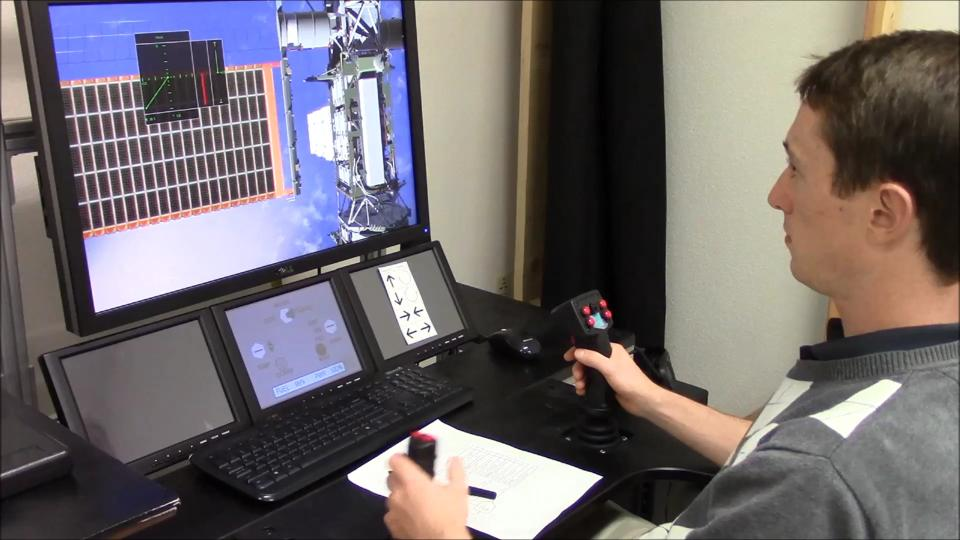
\includegraphics[width=0.8\linewidth]{figures/AR/SAFER_DangerChris.jpg}
        \caption[Simplified Aid for EVA Rescue (SAFER) experiment subject seated in the fixed-base simulator]{A subject from the Simplified Aid for EVA Rescue (SAFER) experiment seated in the fixed-base simulator~\citep{karasinski_real-time_2016}.}
        \label{figure:safersim}
    \end{center}
\end{figure}

Our recent work includes investigations into concurrent bandwidth feedback in a four degree of freedom Simplified Aid for EVA Rescue (SAFER) task~\citep{karasinski_real-time_2016, karasinski_real-time_2017, karasinski_development_2016}.
SAFER is a small propulsive jet pack worn during spacewalks for self-rescue~\citep{Vassigh1998}.
Subjects were tasked with flying a SAFER simulation to perform an inspection of the International Space Station's (ISS) solar arrays.
Subjects were initially placed 40 feet away from the solar array and were asked to close to 30 feet and hold this distance for the remainder of the task.
They could gauge their distance from the solar array using the indicator on the guidance display and the out-the-window display.
Subjects were then asked to inspect four waypoints on the solar array and were given a guidance display for navigation to the waypoints.
Two vertically arranged displays in the simulator were available to complete the task (see Figure~\ref{figure:safersim}).
The primary display contained an out-the-window view of the solar array and, depending on which group the subject was in, one of the guidance displays.
The secondary display located directly below the primary display portrayed information about the subject's current mode, remaining fuel, and a ``comm light.''

\begin{figure}[tb!]
    \begin{center}
        \begin{subfigure}{0.49\textwidth}
            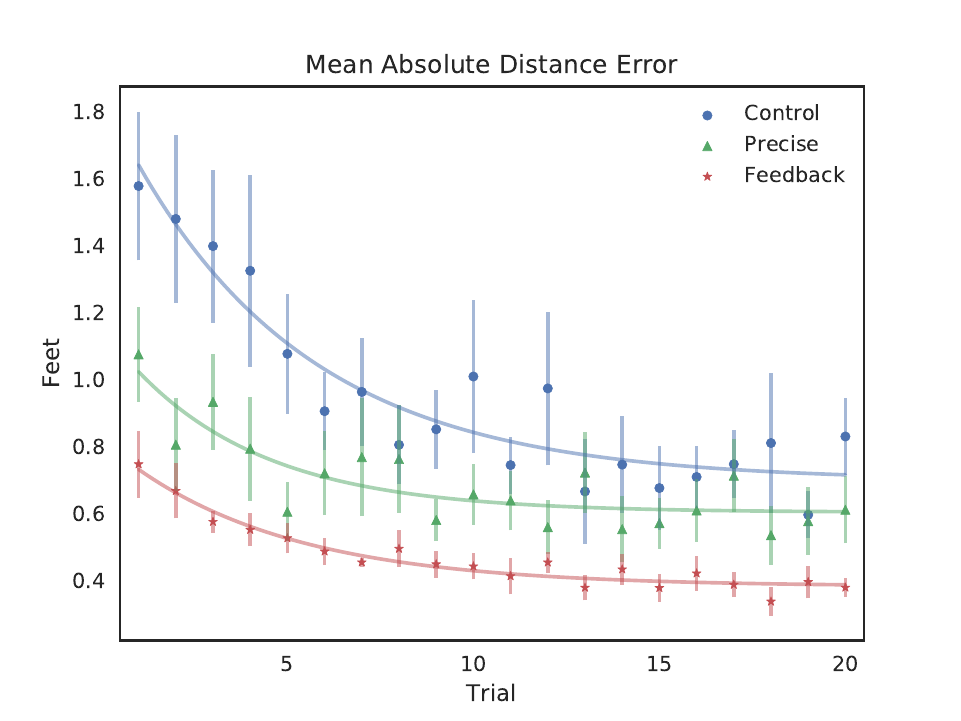
\includegraphics[width=\linewidth]{figures/AR/Group_absDistErr_clean_fit_30.png}
            \caption[Mean absolute distance error]{Mean absolute distance error.}
            \label{figure:saferdistance}
        \end{subfigure}\hfill
        \begin{subfigure}{0.49\textwidth}
            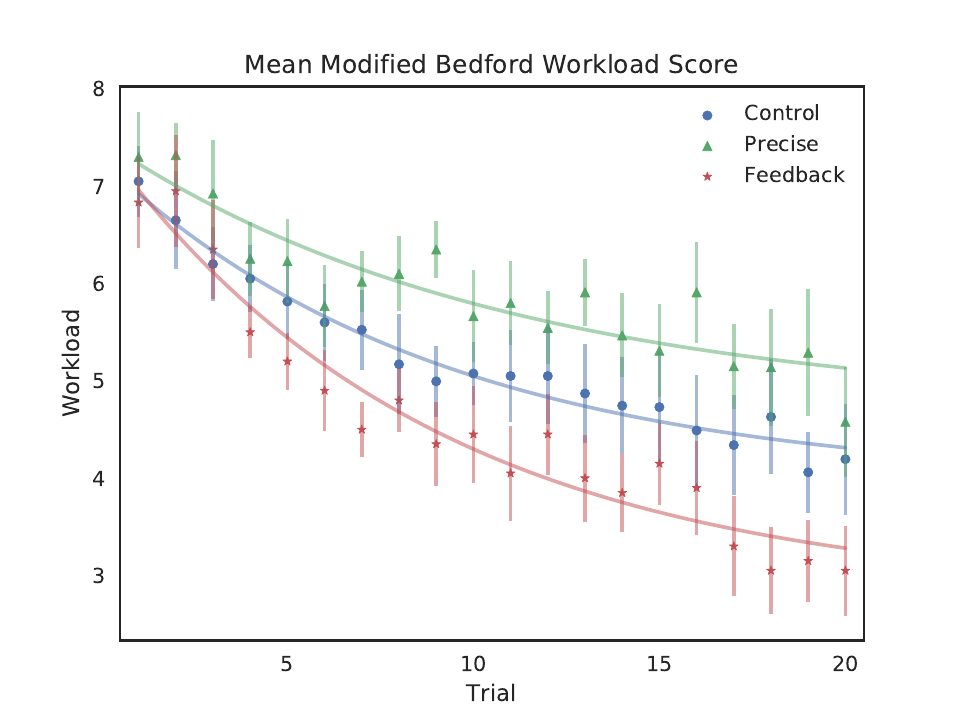
\includegraphics[width=\linewidth]{figures/AR/Group_Workload_fit_30.png}
            \caption[Mean subjective workload rating]{Mean subjective workload rating.}
            \label{figure:saferworkload}
        \end{subfigure}
        \caption[Performance and workload benefits from feedback]{Subjects with concurrent bandwidth feedback (CBF) performed the best (a) and reported the lowest workload (b). Errors are the standard error of the mean~\citep{karasinski_real-time_2016}.}
    \end{center}
\end{figure}

In our experiment, subjects were placed into one of three groups: a control, a high precision augmented feedback group, and a concurrent bandwidth feedback (CBF) group.
Subjects in the high precision group were given an extra significant figure in their guidance display and an analog display which was scaled twice as large (but had half the maximum value) of their flight parameters.
Subjects in the CBF group had two display elements which would change from a green to a red color when the subject's performance was outside a predefined range.
Performance was measured as mean absolute distance error (MAE) and results across trials are shown in Figure~\ref{figure:saferdistance}.
Both treatment groups performed better than the control group, with the CBF group performing the best and having the least error.
The effects that the treatments had on workload was very different than performance, however.
Subjects in the high precision group reported significantly more workload than the control group, while subjects in the CBF group reported significantly less workload than the control group (see Figure~\ref{figure:saferworkload}).
The concurrent bandwidth feedback also had the added benefit of significantly reducing the amount of time required to train the subjects to their maximum skill level.
Subjects with the CBF performed better on their first trial than subjects in the control group did on their last, which was after approximately two hours on the task.

\subsection{Concurrent Bandwidth Feedback}
\begin{figure}[tb]
    \begin{center}
        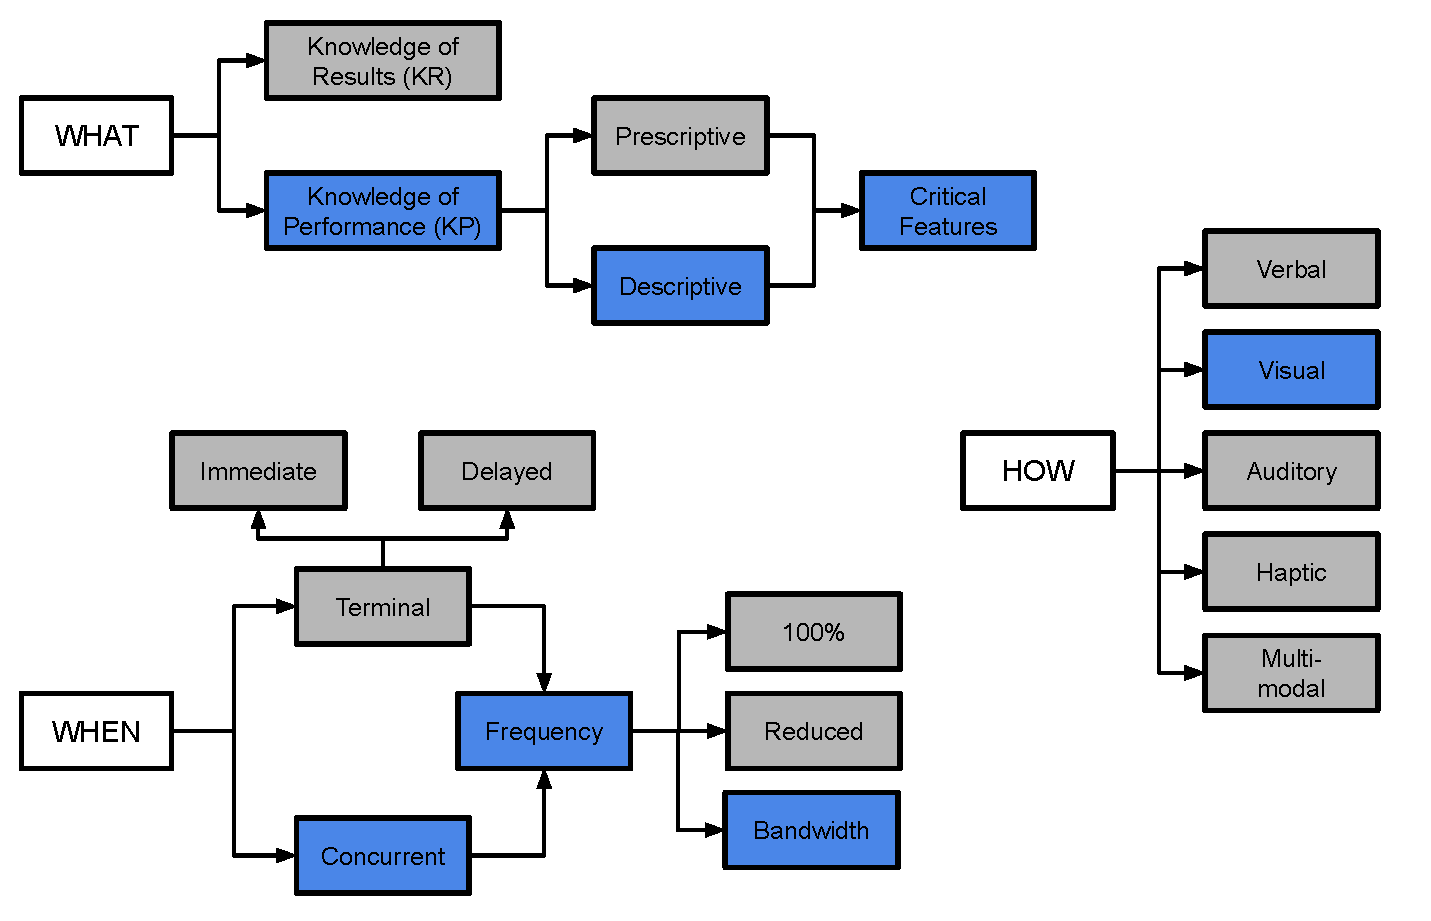
\includegraphics[width=\linewidth]{figures/Introduction/feedbackschematichighlighted.pdf}
        \caption[A schematic of the primary what, when, and how variables that need to be considered when providing augmented feedback]{A schematic of the primary what, when, and how variables that need to be considered when providing augmented feedback, adapted from~\citep{hodges2020skill}. Blue boxes identify the primary feedback considered in this dissertation.}
        \label{figure:afvariables}
    \end{center}
\end{figure}

Through our experimental work with augmented feedback, we have found concurrent bandwidth feedback to be an effective technique to enhance performance without increasing workload.
It is important to carefully consider all aspects of the task when deciding what, when, and how to provide augmented feedback.
While we experimented with different whats, whens, and hows when initially designing the augmented feedback technique presented in this dissertation, we neither completed an exhaustive study, nor did we complete extensive experimental comparisons.
Instead, when designing this feedback, we considered the role of an expert instructor in training a complex skill, such as learning to fly an airplane.
In this instructor model, the trainee has a basic understanding of the task, but the expert instructor can inform them on aspects of the task that they may not be aware of or that they do not have sufficient cognitive margin to attend to.
By pointing at elements on a display or providing verbal feedback, the instructor can identify what aspects of the tasks the trainee needs to pay attention to in real-time.
The instructor chooses some bandwidth of acceptable performance for each aspect of the task, and their role in providing feedback gradually fades away as the trainee becomes more expert in the task.
Figure~\ref{figure:afvariables}, adapted from \citeauthor{hodges2020skill}, presents a schematic of the primary what, when, and how variables that need to be considered when providing augmented feedback.
The choices involved in choosing the what, when, and how to provide this feedback are presented here.

% WHAT
Deciding \textit{what} information to provide to subjects is not trivial, especially when the task contains a large number of relevant variables.
Under the paradigm of the instructor model, we have chosen to highlight elements that are provided in the guidance display rather than add on additional augmented feedback elements.
\citeauthor{sigrist_augmented_2013} states that ``feedback in complex tasks should be prescriptive--that is, feedback should inform the learning on how to correct the error--rather than descriptive (i.e., information about occurrence of an error)'', though we have found that feedback that is purely descriptive can be effective for training complex flight tasks.
Many of the tasks considered by \citeauthor{sigrist_augmented_2013} were targeting specific, short movements or related to sports tasks, however, which do not normally include guidance displays like those found in aerospace tasks.
As these guidance displays are prevalent in the aerospace domain and our subjects were trained in how to use them to accomplish their tasks, it may be that prescriptive feedback is not necessary in this case.
The subjects are already aware of their errors, and the descriptive feedback provided by the concurrent bandwidth feedback simply provides a descriptive of what the most temporally relevant error is.
It has also been suggested that the motor task is relatively simple for flight and driving tasks, and that most of the difficulty associated with the task comes from the high levels of cognitive demand~\citep{doi:10.1080/00222899709600829}.
Under this consideration, simply knowing which error to focus on at any given time may be sufficient for improving performance and could be responsible for the reduction in workload we observed in our previous SAFER study.
In any case, the type of skill and task is certainly ``a critical factor in determining the effectiveness and the appropriateness of the corrective feedback types''~\citep{Tzetzis2008}.

% WHEN
Choosing \textit{when} to provide feedback can be one of the most import aspects of augmented feedback.
Providing feedback terminally, when the task is over, may be too late to provide a performance benefit, while providing feedback concurrently, in real-time as the task is being executed, can overwhelm the trainee.
\citeauthor{sigrist_augmented_2013} note that ``it seems that the more complex the task, the more the trainee can profit from concurrent feedback.''
When considering the instructor model approach, we chose to focus on concurrent feedback.
% ``Thus, the frequency of feedback should decrease with increasing skill level--that is, with decreasing functional task complexity--to further facilitate motor learning.
% Functional task complexity depends of the current individual skill level and changes during the learning process, whereas nominal task complexity remains invariant.''
It is well established that the frequency of feedback should decrease with increased skill level~\citep{doi:10.3200/JMBR.36.2.212-224, timmermans_technology-assisted_2009, Wulf2002, doi:10.1080/00222899809601335}.
% ``Reduced feedback frequency--that is, fading feedback--seems beneficial for both terminal feedback and concurrent feedback''
It has also been shown that fading feedback, which appears less frequently over time, is beneficial for both terminal and concurrent feedback~\citep{CROWELL201178, KOVACS2011311}.
By reducing the frequency of feedback, subjects learn to develop their internal models of the task and identify their own task errors, reducing their dependency of the feedback.
The role of the instructor should similarly decrease over time as trainees become more proficient.
This led us to the concept of presenting concurrent feedback when performance variables deviated outside of an acceptable bandwidth.
Bandwidth feedback, however, is not without its own difficulties.
Several authors have noted that ``[b]andwidth feedback has been shown to be effective; however, setting the error threshold is not trivial''~\citep{sigrist_augmented_2013, timmermans_technology-assisted_2009, RIBEIRO2011231}.
This issue has usually been associated with terminal bandwidth feedback, where it is challenging to decide what types of descriptive summary statistics are appropriate and what bandwidths are sufficient.
By instead choosing to present the feedback concurrently we can use an operational limit or chosen bandwidth of acceptable performance, which can make the choice of setting the error threshold simpler.

% HOW (and where)
The \textit{how} of presenting feedback has largely focused on which modality (or modalities) to use.
Under the paradigm of the instructor model, we considered the verbal and visual modalities.
Many aerospace tasks, however, involve significant secondary tasks in the form of managing interactions with air traffic control or communicating over other voice loops.
With this consideration, the concurrent bandwidth we developed was exclusively visual, involving color changes on the guidance display. 
One advantage of focusing on the visual modality is that this is where a majority of research in augmented feedback has focused, allowing us to more easily compare between other research studies.

In summary, concurrent bandwidth feedback is provided to an operator in real-time when a signal deviates out of a predefined range.
In this work, the feedback is always displayed visually and changes the color of an already existing element of the display.
Figure~\ref{fig:cbf} illustrates the process of taking the signal from a task relevant feature and applying this technique.
For example:
\begin{enumerate}
\item A task relevant signal is identified.
Figure~\ref{fig:signal} shows an example signal, the pitch disturbance from the aircraft flight task presented in Chapter~\ref{chapter:aircraftfeedback}.
\item An operationally relevant performance bandwidth is identified.
Figure~\ref{fig:signal_w_bandwidth} shows an example bandwidth of acceptable performance.
\item Visual feedback is applied to an existing part of the display and presented to the operator concurrently.
Figure~\ref{fig:signal_w_feedback} shows an example of feedback that would be presented to an operator.
In this example, an element of the display would change from green (acceptable performance) to red (unacceptable performance) when the operator deviates outside of the acceptable pitch range.
\end{enumerate}

\begin{figure}[p]
    \begin{center}
        \begin{subfigure}{0.80\textwidth}
            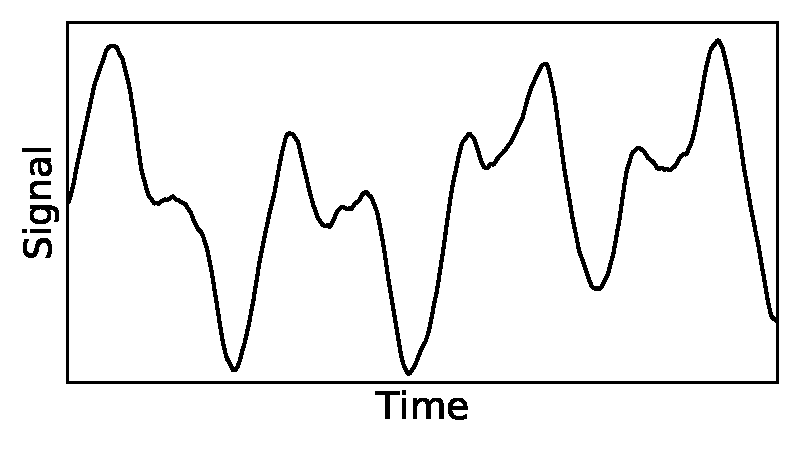
\includegraphics[width=\linewidth]{figures/Introduction/signal.pdf}
            \caption[The signal of a task critical feature]{The signal of a task critical feature.}
            \label{fig:signal}
        \end{subfigure}\hfill
        \begin{subfigure}{0.80\textwidth}
            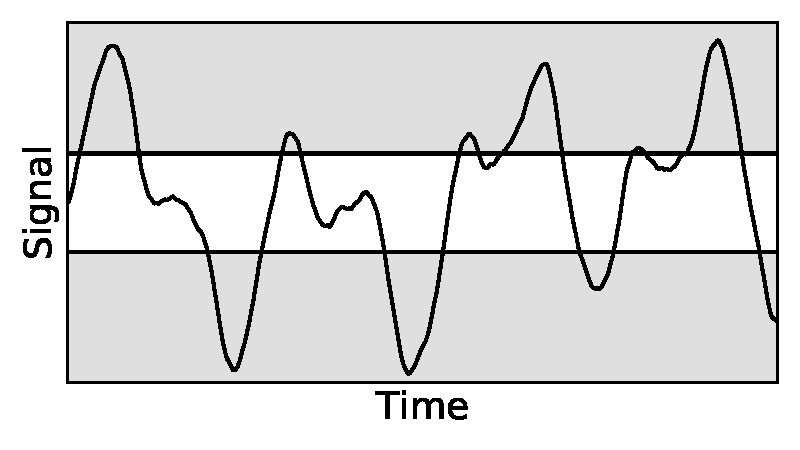
\includegraphics[width=\linewidth]{figures/Introduction/signal_w_bandwidth.pdf}
            \caption[The signal with an operationally relevant bandwidth]{The signal with an operationally relevant bandwidth.}
            \label{fig:signal_w_bandwidth}
        \end{subfigure}\hfill
        \begin{subfigure}{0.80\textwidth}
            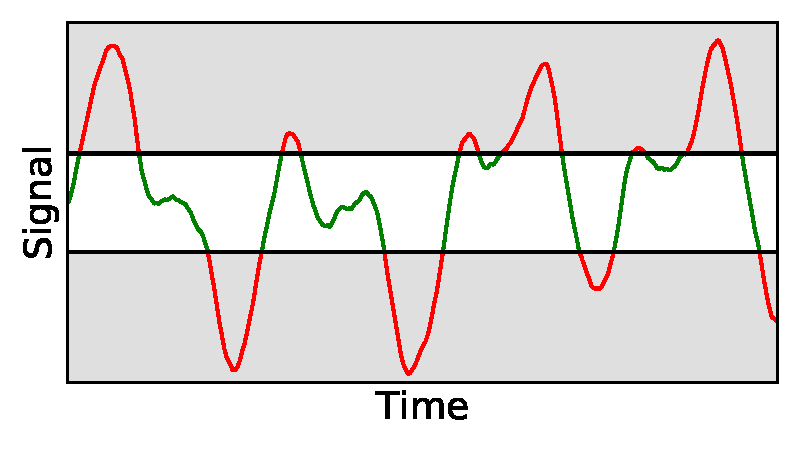
\includegraphics[width=\linewidth]{figures/Introduction/signal_w_feedback.pdf}
            \caption[The signal with concurrent bandwidth feedback applied]{The signal with concurrent bandwidth feedback applied.}
            \label{fig:signal_w_feedback}
        \end{subfigure}
        \caption[The implementation of concurrent bandwidth feedback to a task critical feature]{The implementation of concurrent bandwidth feedback to a task critical feature.}
        \label{fig:cbf}%
    \end{center}
\end{figure}

\subsection{Workload}
\textbf{\color{red} Briefly discuss the Modified Bedford Workload Score and the NASA-TLX.}

\citep{roscoe_subjective_1990, hart_development_1988, hart_nasa-task_2006}

\subsection{Pilot Modeling}
\label{background:pilotmodeling}
\begin{figure}[tb]
    \begin{center}
        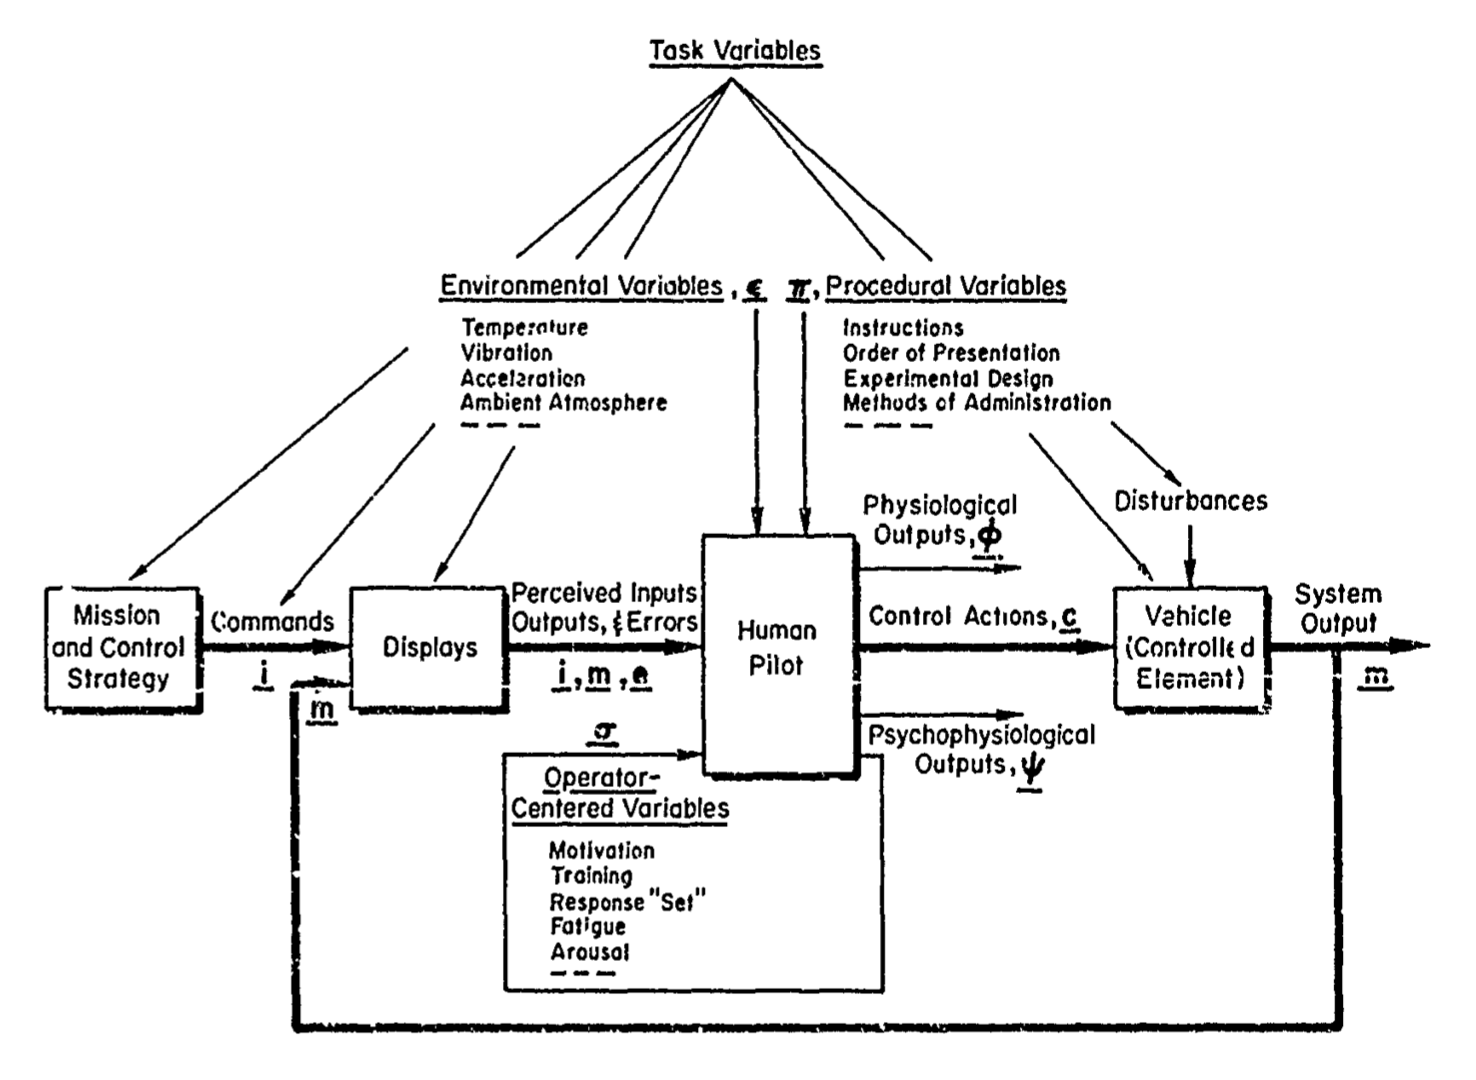
\includegraphics[width=0.8\linewidth]{figures/Introduction/Screen_Shot_2018-07-25_at_10_37_08_AM.png}
        \caption[Variables affecting the pilot/vehicle system]{Variables affecting the pilot/vehicle system, from~\citet{mcruer_mathematical_1974}.}
        \label{figure:mcruer1974}
    \end{center}
\end{figure}

In addition to popularizing the concept of feedback, the creation of control theory in the early 1940s also provided the tools required for the mathematical modeling of the human pilot.
At the time, new weapons were being created for World War 2 which could only be used effectively with trained operators working with a machine.
While it was thought that a human could be viewed as a unique kind of servomechanism in the control feedback loop, it was still unclear what factors affected human performance.
Early work by Tustin and others extended the control theory framework and applied these theories to actual human operators~\citep{tustin1944investigation}.
Particular interest was focused on ``attempt[ing] to find the laws of relationship of movement and error.
In particular, it was hoped that this relationship [would] be approximately linear and so permit well developed theory of `linear servomechanisms' to be applied to manual control in the same way as it applies to automatic following~\citep{tustin1944investigation}.''
This would allow for the prediction of human performance and the ability to predict the limits of human control.

These early works were summarized in \citeauthor{mcruer_dynamic_1957}'s report, ``Dynamic Response of Human Operators.''
This work evaluated measurements for single-input/single-output (SISO) manual control systems and developed predictive models consistent with this data.
Indeed, \citeauthor*{mcruer_dynamic_1957} write, ``[i]t is possible, without doing violence to the data, to obtain describing functions which are generally applicable to the results of the many diverse experiments.''
The report concludes by describing a hypothetical transfer function of the human operator which includes a time delay, a neuromuscular lag, and a gain.
McRuer's early model of the complete pilot/vehicle system is presented in Figure~\ref{figure:mcruer1974}.
McRuer revisited these results in \citeyear{mcruer_mathematical_1974}, after three decades of supporting engineering and experimental psychology experiments and was able to further generalize these results to a wide variety of system dynamics.
In his study, McRuer completed a detailed analysis which included the human response to proportional, rate/velocity, and acceleration type controlled element dynamics, see Table~\ref{table:mcruer1974a}.
The result of this report was the now famous ``crossover model,'' which relates the operator and controlled element transfer characteristics by the equation
\begin{align}
    Y_c(jw) Y_p(jw) = \dfrac{w_c e^{-jw \tau_e}}{jw}
\end{align}
where $Y_c$ is the controlled element transfer function, $Y_p$ is the approximate human operator transfer function, $w_c$ is the crossover frequency, and $\tau_e$ is the effective time delay of the pilot.
The crossover model is so named as it allows for linear behavior at approximately -20 dB/decade slope in the region of the crossover frequency.
The approximate human operator response to several controlled element transfer functions and their combined open-loop transfer function are presented in Table~\ref{table:mcruer1974b}.
Modeling the human pilot with the crossover enabled a more complete view of the complete pilot/vehicle system and allowed for human factors recommendations towards the design of new vehicles.
Even today, the crossover model is used as the standard for describing pilot/vehicle systems at the crossover frequency~\citep{mcruer_human_1965, mcruer_mathematical_1974, xu_review_2017}.

\begin{table}[tb]
    \centering
    \includetable{intro-idealized-control-elements.tex}
    \caption[Example Applications of Idealized Controlled Element Forms]{Example Applications of Idealized Controlled Element Forms, adapted from~\citet{mcruer_mathematical_1974}.}
    \label{table:mcruer1974a}
\end{table}

\begin{table}[tb]
    \centering
    \includetable{intro-human-operator-characteristics.tex}
    \caption[Summary of Human Operator Approximate Characteristics]{Summary of Human Operator Approximate Characteristics, adapted from~\citet{mcruer_mathematical_1974}.}
    \label{table:mcruer1974b}
\end{table}

The continued demand for human pilot models for use in informing vehicle design, as well predicting, preventing, and explaining accidents has led to a variety of more complex pilot models since the creation of the crossover model.
A recent review by Xu et al. in 2017 surveyed the state of the art in human pilot modeling and grouped existing models into three classes of models based on: control theory, human physiology, and intelligence techniques~\citep{xu_review_2017}.
Classical models based on control theory include the McRuer crossover model and optimal control models by Kleinman et al. developed in the early 1970s~\citep{kleinman_optimal_1970, baron_optimal_1970}.
Models based on human physiology were developed to understand human pilot perception and control behavior, and include the Hess structural model~\citep{hess_structural_1980, hess_model_1990, hess_unified_1997}, Hosman's descriptive model~\citep{hosman_pilots_nodate, hosman_pilots_1999}, and the biodynamic model~\citep{griffin_validation_2001}.
Recent intelligence models take advantage of techniques including fuzzy control and neural networks~\citep{zaychik_conspectus_2006, gestwa_modelling_2003}.
Of these three overarching sets of models, the models based on human physiology are of the greatest interest here.

\begin{figure}[tb!]
    \begin{center}
        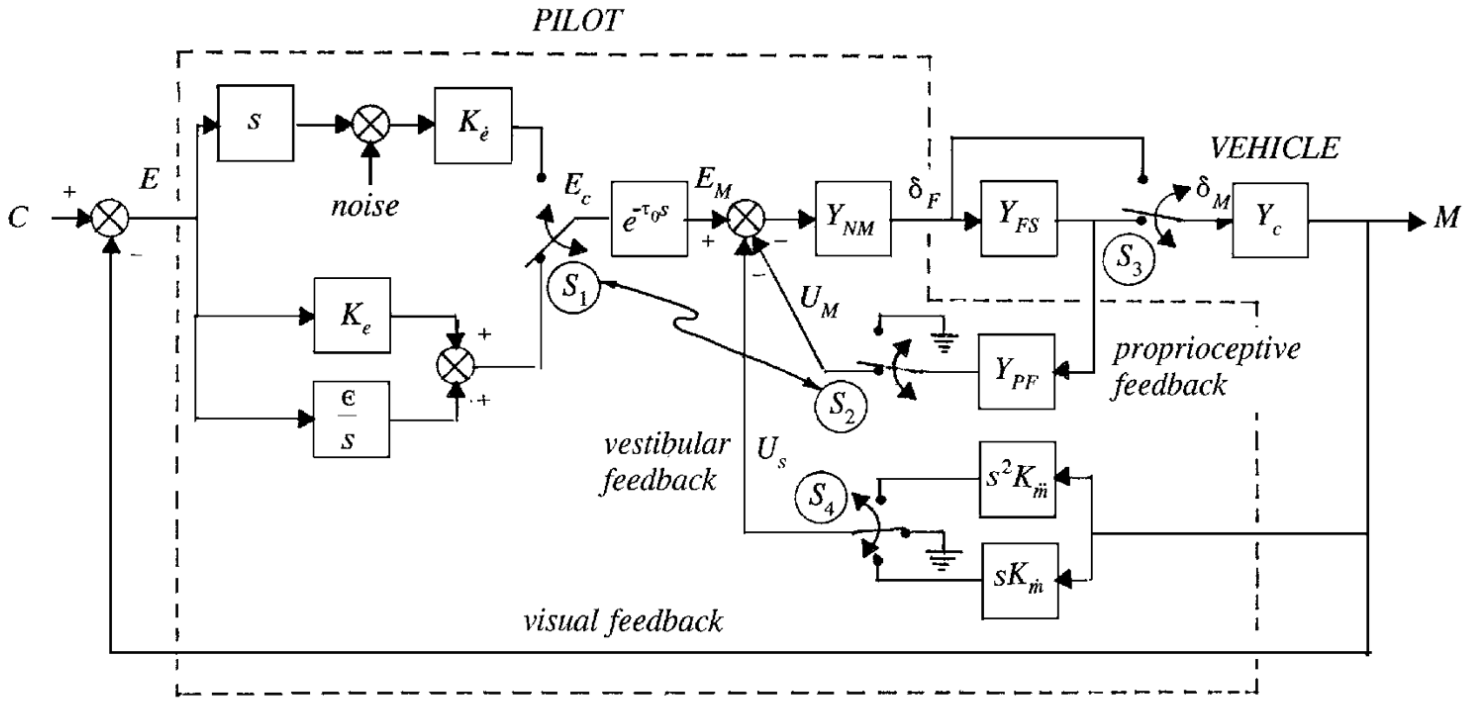
\includegraphics[width=0.8\linewidth]{figures/Introduction/Screen_Shot_2018-07-31_at_11_21_44_AM.png}
        \caption[The Hess Structural Model of the Human Pilot]{The Hess Structural Model of the Human Pilot, from~\citet{hess_unified_1997}.}
        \label{figure:structuralmodel}
    \end{center}
\end{figure}

While the crossover model was very successful in predicting pilot behavior, it it did not attempt ``to describe the underlying structure which contributes to human pilot dynamics~\citep{hess_structural_1980}.''
For this reason, the Hess Structural Model is of interest due to the incorporation of multiple sensory channels and models of visual acuity and the time-varying human pilot~\citep{hess_modeling_2009}.
The Structural Model includes the effects of the neuromuscular system, the force-feel characteristics of the input device, and the contributions of proprioceptive, vestibular, and visual feedback, see Figure~\ref{figure:structuralmodel}.
One of the key strengths of the Structural Model is the relatively small number of free parameters that need to be set to predict pilot performance.
The model has been used in predicting and evaluating handling qualities and pilot-induced oscillation rating levels for helicopters, Boeing 747, Lockheed C-5A, and twin ducted-fan aircraft~\citep{hess_analytical_2013, andreea-irina_prediction_2014, grant_handling_2015}.
Hess has also investigated how pilot control characteristics change with time due to flight anomalies, changing flight dynamics, and sudden increases in task demand~\citep{hess_modeling_2009, hess_modeling_2016}.
The results of this model have been compared to the results of a human-in-the-loop simulation for a well-trained subject and showed good comparison~\citep{hess_modeling_2016}.
Recent work from Bachelder et al. has included modifications to the Structural Model to link pilot performance and workload and to enable the modeling of pulsive pilot behavior~\citep{bachelder_modeling_2017, bachelder_linking_2018}.

\subsection{Summary}
Concurrent bandwidth feedback has been used in a large variety of motor control tasks and has generally been found to improve performance.
Until recently, however, only simple tasks such as physical movements or low-dimensional pursuit tasks have been investigated.
More recent works, including the lane-keeping task by \citeauthor{de_groot_effect_2011}, and our previous work with the SAFER task, have indicated that concurrent bandwidth feedback can also be quite effective for complex tasks~\citep{karasinski_real-time_2017}.
Unlike simple tasks, in which the guidance hypothesis dominates when feedback is removed, there is some evidence that concurrent bandwidth feedback can be removed after training without a loss of performance.
The decrease in required learning time, improved performance, and decreased workload seen in the SAFER task show that concurrent bandwidth feedback may prove to be most useful very early in training when subjects are first exposed to complex, highly dynamic tasks.
As concurrent bandwidth feedback can improve performance without an increase in workload, it may prove a useful technique for training other complex manual control tasks.

There has been considerable improvement in the field of pilot modeling since McRuer's crossover model, especially with models that incorporate human physiology.
The Structural Model, in particular, has been very effective in predicting pilot performance, handling qualities, pilot-induced oscillation rating levels, and workload for a variety of system dynamics.
None of these pilot models, however, are able to include the effects of concurrent bandwidth feedback.
The performance improving effects of this feedback, seen throughout the literature, make this a compelling feature to be incorporated into a pilot model.

This literature review covered the development of the augmented feedback, focusing on examples of concurrent and bandwidth feedback.
Extra focus was spent on cases where augmented feedback techniques were applied to aerospace related tasks.
Additionally, this review covered human performance models applied to piloted aircraft and flight-like tasks.

\section{Research Questions}
\label{sec:intro_questions}
We are interested in measuring, modeling, and predicting the effects of concurrent bandwidth feedback (CBF) on human performance in complex manual control tasks.
To this end, this proposed research includes two research aims.
These aims build on each other, starting with a compensatory tracking task, extending to surface electromyography and aircraft flight tasks, and finishing with a theoretical model.

We set out to accomplish two aims with the research included in this dissertation.
This dissertation contains the results of human-in-the-loop subject testing experiments which were designed to understand the effects of concurrent bandwidth feedback.
Using the data from these experiments, the structural model has modified to integrate the effects of this feedback into a human performance model.
To investigate the two Aims outlined below, we completed four experiments and the development of a model.

\begin{description}[align=left]
    \item [Aim One] Investigate the effects of concurrent bandwidth feedback on human performance and workload in complex manual control tasks.
    \item [Aim Two] Extend the Hess Structural Model of the human pilot to include the effects of concurrent bandwidth feedback.
\end{description}

There are several research questions that we were interested in answering by completing these aims, which included:
\begin{enumerate}
    \item Can concurrent bandwidth feedback improve performance of complex manual control tasks?
          \begin{enumerate}
              \item Can CBF reduce the required training time to peak performance?
              \item Can CBF be removed after reaching peak performance without reducing subject performance (i.e., does the guidance hypothesis not hold)?
              \item Does CBF improve performance in transfer of training tasks?
              \item Can performance be increased without increasing workload?
          \end{enumerate}
    \item Can we develop a model of human performance which includes the effects of concurrent bandwidth feedback?
          \begin{enumerate}
              \item Can we use this model to estimate operational limits?
          \end{enumerate}
\end{enumerate}

\section{Summary}
We have introduced our goals and motivation for the design and use of the concurrent bandwidth feedback, a technique for enhancing motor control training without inducing higher levels of workload.
The background for the experimental work has been described and the open research questions that we explore in this work have been summarized.
In the following chapters, we first present a systematic assessment of current and upcoming human automation/robotic integration technologies and research topics (Chapter~\ref{chapter:tradestudy}), then report on four experiments involving augmented feedback (Chapters~\ref{chap:3dtracking}-\ref{chapter:aircraftfeedback}), propose a theoretical model which explains the observed effects of the feedback (Chapter~\ref{chapter:modeling}), and summarize our findings and proposed future work (Chapter~\ref{chap:conclusion}).
